% figure1_pair_chipflow.tex — (a) pikv workflow + (b) 3-column mechanism view.
% Round-3 redesign:
%   - Middle column carries the RepairKV operator (score, top-K, promote) and
%     receives the signal from above; eliminates curved arrows that crossed
%     GPU active.
%   - Style harmonized with (a): identical box/store/active styles, fonts.
%   - More host chips for symmetry (4 sub-rows of 6).
%   - All arrows are short straight segments; no curves.
% Shared preamble for standalone Figure 1 variants.
\documentclass[border=8pt,tikz]{standalone}
\usepackage{amsmath}
\usepackage{amssymb}
\usepackage{tikz}
\usetikzlibrary{arrows.meta,positioning,calc,fit,shapes.geometric,backgrounds}
\usepackage{xcolor}
\usepackage[T1]{fontenc}
\usepackage{mathptmx}
\newcommand{\repairkv}{\textsc{RepairKV}}
\newcommand{\bbase}{\ensuremath{B_{\mathrm{base}}}}
\newcommand{\bmatch}{\ensuremath{B_{\mathrm{match}}}}

\begin{document}
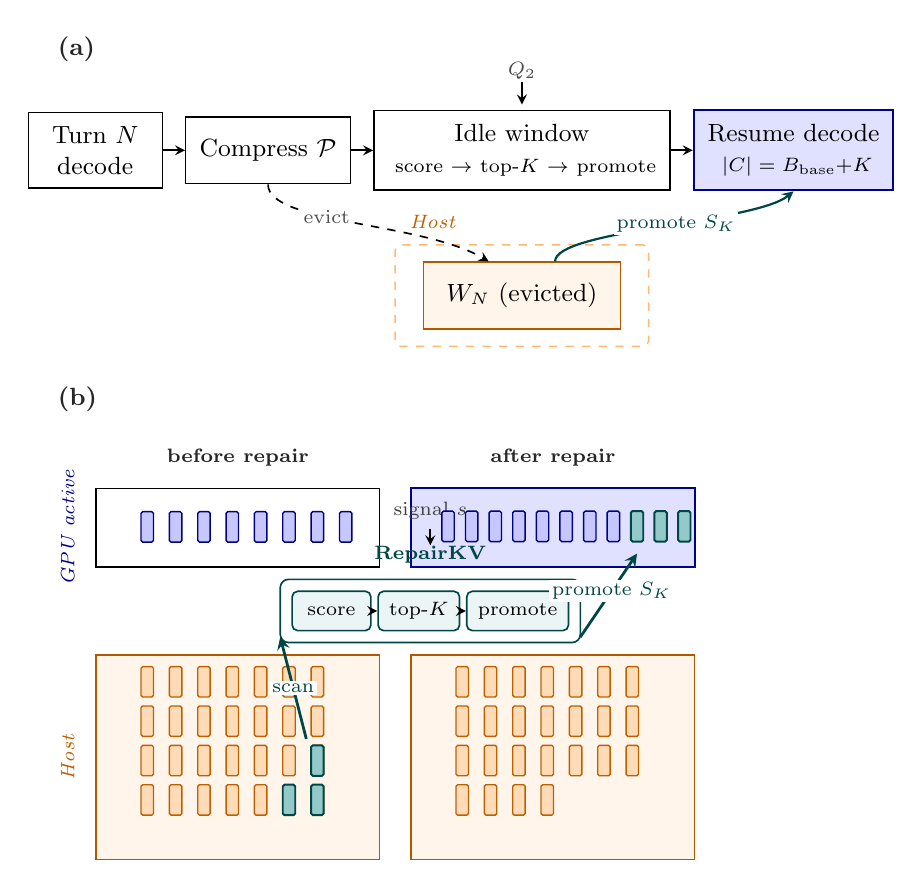
\begin{tikzpicture}[
  >=latex, line width=0.4pt,
  font=\small,
  % --- shared styles between (a) and (b) ---
  box/.style={draw=black, fill=white, line width=0.5pt,
              inner sep=5pt, align=center, minimum height=0.85cm},
  active/.style={box, fill=blue!12, draw=blue!55!black, line width=0.7pt},
  store/.style={box, fill=orange!8, draw=orange!70!black},
  arr/.style={->, line width=0.6pt, draw=black, >=stealth},
  promarr/.style={->, line width=0.8pt, draw=teal!55!black, >=stealth},
  arrlabel/.style={font=\scriptsize, text=black!70, fill=white, inner sep=1pt},
  groupbox/.style={draw=orange!55, dashed, line width=0.5pt, rounded corners=2pt},
  grouplabel/.style={font=\scriptsize\itshape, text=orange!75!black},
  panellabel/.style={font=\bfseries\small, text=black!85},
  % --- chip styles ---
  chip/.style={rounded corners=0.6pt, minimum width=4.5pt, minimum height=11pt,
               inner sep=0pt, line width=0.5pt},
  gpuchip/.style={chip, draw=blue!50!black, fill=blue!22},
  hostchip/.style={chip, draw=orange!75!black, fill=orange!28},
  promchip/.style={chip, draw=teal!55!black, fill=teal!42, line width=0.7pt},
  rkvbox/.style={draw=teal!55!black, fill=teal!8, line width=0.6pt,
                 rounded corners=2pt, inner sep=4pt, align=center,
                 font=\scriptsize, minimum width=1.7cm, minimum height=0.5cm},
  bigpromarr/.style={->, line width=1.0pt, draw=teal!55!black, >=stealth},
  rowlabel/.style={font=\itshape\scriptsize}
]
  % =================================================================
  % Panel (a) — pikv block diagram
  % =================================================================
  \node[panellabel, anchor=south west] at (0, 4.4) {(a)};

  \node[box, minimum width=1.7cm] (dN) at (0.6, 3.4) {Turn $N$\\decode};
  \node[box, minimum width=1.6cm, right=8pt of dN] (cmp) {Compress~$\mathcal{P}$};
  \node[box, minimum width=2.5cm, right=8pt of cmp] (idle)
       {Idle window\\{\scriptsize{} score~$\to$~top-$K$~$\to$~promote}};
  \node[active, minimum width=1.9cm, right=8pt of idle] (resume)
       {Resume decode\\{\scriptsize{} $|C|=\bbase{+}K$}};

  \draw[arr] (dN) -- (cmp);
  \draw[arr] (cmp) -- (idle);
  \draw[arr] (idle) -- (resume);

  \draw[arr] ([yshift=10pt]idle.north) -- ([yshift=2pt]idle.north);
  \node[arrlabel, anchor=south] at ([yshift=10pt]idle.north) {$Q_2$};

  \node[store, minimum width=2.5cm, below=0.9cm of idle] (wn) {$W_N$ (evicted)};
  \node[groupbox, fit=(wn), inner xsep=10pt, inner ysep=6pt] (hgroup) {};
  \node[grouplabel, anchor=south west]
       at ([xshift=2pt, yshift=2pt]hgroup.north west) {Host};

  \draw[arr, dashed]
       (cmp.south) .. controls ([yshift=-0.5cm]cmp.south)
                              and ([yshift=0.5cm]wn.north west) ..
       ([xshift=-12pt]wn.north)
       node[arrlabel, pos=0.4] {evict};

  \draw[promarr]
       ([xshift=12pt]wn.north) .. controls ([xshift=12pt, yshift=0.4cm]wn.north)
                                          and ([xshift=-0.5cm, yshift=-0.4cm]resume.south) ..
       (resume.south)
       node[arrlabel, text=teal!55!black, pos=0.55] {promote~$S_K$};

  % =================================================================
  % Panel (b) — Before/After columns + RepairKV pill in the row gap.
  %   Two cells per row, with a horizontal RepairKV pill sitting in the
  %   inter-row gap between them. Short straight arrows: host -> pill,
  %   pill -> gpu. Signal s enters pill from above.
  % =================================================================
  \node[panellabel, anchor=south west] at (0, -0.05) {(b)};

  % Cell layout aligned with (a) extent (x=0.6 to ~8.6), wider row gap to
  % accommodate the operator pill.
  \node[box, minimum width=3.6cm, minimum height=1.0cm,
        anchor=south west] (gpuB) at (0.6, -1.9) {};
  \node[active, minimum width=3.6cm, minimum height=1.0cm,
        anchor=south west] (gpuA) at (4.6, -1.9) {};
  \node[store, minimum width=3.6cm, minimum height=2.6cm,
        anchor=north west] (hostB) at (0.6, -3.0) {};
  \node[store, minimum width=3.6cm, minimum height=2.6cm,
        anchor=north west] (hostA) at (4.6, -3.0) {};

  % Tier row labels
  \node[rowlabel, text=blue!55!black, anchor=south, rotate=90]
       at ([xshift=-4pt]gpuB.west) {GPU active};
  \node[rowlabel, text=orange!75!black, anchor=south, rotate=90]
       at ([xshift=-4pt]hostB.west) {Host};

  % Column titles
  \node[font=\bfseries\scriptsize, text=black!85, anchor=south]
       at ([yshift=4pt]gpuB.north) {before repair};
  \node[font=\bfseries\scriptsize, text=black!85, anchor=south]
       at ([yshift=4pt]gpuA.north) {after repair};

  % --- RepairKV pill: horizontal, sitting in the row gap (y = -2.45) ---
  % Three sub-modules side-by-side: score -> top-K -> promote.
  \node[rkvbox, anchor=center, minimum width=1.0cm] (mscore)
        at (3.6, -2.45) {score};
  \node[rkvbox, anchor=west, minimum width=0.8cm] (mselect)
        at ([xshift=2pt]mscore.east) {top-$K$};
  \node[rkvbox, anchor=west, minimum width=1.0cm] (mpromote)
        at ([xshift=2pt]mselect.east) {promote};
  \draw[arr] (mscore.east)  -- (mselect.west);
  \draw[arr] (mselect.east) -- (mpromote.west);

  % Encompass the three modules in a translucent RepairKV "frame"
  \node[draw=teal!55!black, line width=0.6pt, rounded corners=3pt,
        fit=(mscore)(mpromote), inner xsep=4pt, inner ysep=4pt] (rkvframe) {};
  \node[font=\scriptsize\bfseries, text=teal!55!black, anchor=south]
       at ([yshift=2pt]rkvframe.north) {\repairkv{}};

  % --- signal s entering RepairKV from above ---
  \draw[arr] ([yshift=18pt]rkvframe.north) -- ([yshift=12pt]rkvframe.north);
  \node[font=\scriptsize, text=black!75, anchor=south]
       at ([yshift=18pt]rkvframe.north) {signal $s$};

  % --- GPU before chips: 8 blue (denser to match host symmetry) ---
  \foreach \i in {1,...,8}{
    \pgfmathsetmacro{\xc}{0.36*\i + 0.30}
    \node[gpuchip] at ([xshift=\xc cm, yshift=-0.5cm]gpuB.north west) {};
  }
  % --- GPU after chips: 8 blue + 3 teal (right end) ---
  \foreach \i in {1,...,8}{
    \pgfmathsetmacro{\xc}{0.30*\i + 0.18}
    \node[gpuchip] at ([xshift=\xc cm, yshift=-0.5cm]gpuA.north west) {};
  }
  \foreach \i in {1,2,3}{
    \pgfmathsetmacro{\xs}{0.30*8 + 0.30*\i + 0.18}
    \node[promchip] (gpuTeal\i) at ([xshift=\xs cm, yshift=-0.5cm]gpuA.north west) {};
  }

  % --- Host before: 4 sub-rows of 7 chips = 28 chips, 3 teal at right ---
  \foreach \i in {1,...,7}{
    \foreach \r in {0,1,2,3}{
      \pgfmathsetmacro{\xh}{0.36*\i + 0.30}
      \pgfmathsetmacro{\yh}{-0.35 - 0.50*\r}
      \node[hostchip] at ([xshift=\xh cm, yshift=\yh cm]hostB.north west) {};
    }
  }
  \pgfmathsetmacro{\xPa}{0.36*6 + 0.30} \pgfmathsetmacro{\yPa}{-0.35 - 0.50*3}
  \pgfmathsetmacro{\xPb}{0.36*7 + 0.30} \pgfmathsetmacro{\yPb}{-0.35 - 0.50*2}
  \pgfmathsetmacro{\xPc}{0.36*7 + 0.30} \pgfmathsetmacro{\yPc}{-0.35 - 0.50*3}
  \node[promchip] (hostTealA) at ([xshift=\xPa cm, yshift=\yPa cm]hostB.north west) {};
  \node[promchip] (hostTealB) at ([xshift=\xPb cm, yshift=\yPb cm]hostB.north west) {};
  \node[promchip] (hostTealC) at ([xshift=\xPc cm, yshift=\yPc cm]hostB.north west) {};

  % --- Host after: 25 chips (3 fewer; rightmost positions empty) ---
  \foreach \i in {1,...,7}{
    \foreach \r in {0,1,2}{
      \pgfmathsetmacro{\xh}{0.36*\i + 0.30}
      \pgfmathsetmacro{\yh}{-0.35 - 0.50*\r}
      \node[hostchip] at ([xshift=\xh cm, yshift=\yh cm]hostA.north west) {};
    }
  }
  \foreach \i in {1,...,4}{
    \pgfmathsetmacro{\xh}{0.36*\i + 0.30}
    \node[hostchip] at ([xshift=\xh cm, yshift=-1.85cm]hostA.north west) {};
  }

  % --- Flow arrows: short, straight, both up-right diagonals ---
  % Host (before, top-right) -> pill score (left)
  \draw[bigpromarr] ([yshift=2pt, xshift=-4pt]hostTealB.north)
                    -- ([xshift=-4pt, yshift=-2pt]mscore.south west)
       node[arrlabel, text=teal!55!black, pos=0.5, font=\scriptsize] {scan};
  % pill promote (right) -> GPU (after, bottom-left)
  \draw[bigpromarr] ([xshift=4pt, yshift=-2pt]mpromote.south east)
                    -- ([yshift=-4pt]gpuTeal1.south)
       node[arrlabel, text=teal!55!black, pos=0.55, font=\scriptsize] {promote $S_K$};
\end{tikzpicture}
\end{document}
